\documentclass[]{article}
\usepackage{lmodern}
\usepackage{amssymb,amsmath}
\usepackage{ifxetex,ifluatex}
\usepackage{fixltx2e} % provides \textsubscript
\ifnum 0\ifxetex 1\fi\ifluatex 1\fi=0 % if pdftex
  \usepackage[T1]{fontenc}
  \usepackage[utf8]{inputenc}
\else % if luatex or xelatex
  \ifxetex
    \usepackage{mathspec}
  \else
    \usepackage{fontspec}
  \fi
  \defaultfontfeatures{Ligatures=TeX,Scale=MatchLowercase}
\fi
% use upquote if available, for straight quotes in verbatim environments
\IfFileExists{upquote.sty}{\usepackage{upquote}}{}
% use microtype if available
\IfFileExists{microtype.sty}{%
\usepackage{microtype}
\UseMicrotypeSet[protrusion]{basicmath} % disable protrusion for tt fonts
}{}
\usepackage[margin=1in]{geometry}
\usepackage{hyperref}
\hypersetup{unicode=true,
            pdftitle={POLS 904 Final Project},
            pdfauthor={Jiacheng He},
            pdfborder={0 0 0},
            breaklinks=true}
\urlstyle{same}  % don't use monospace font for urls
\usepackage{longtable,booktabs}
\usepackage{graphicx,grffile}
\makeatletter
\def\maxwidth{\ifdim\Gin@nat@width>\linewidth\linewidth\else\Gin@nat@width\fi}
\def\maxheight{\ifdim\Gin@nat@height>\textheight\textheight\else\Gin@nat@height\fi}
\makeatother
% Scale images if necessary, so that they will not overflow the page
% margins by default, and it is still possible to overwrite the defaults
% using explicit options in \includegraphics[width, height, ...]{}
\setkeys{Gin}{width=\maxwidth,height=\maxheight,keepaspectratio}
\IfFileExists{parskip.sty}{%
\usepackage{parskip}
}{% else
\setlength{\parindent}{0pt}
\setlength{\parskip}{6pt plus 2pt minus 1pt}
}
\setlength{\emergencystretch}{3em}  % prevent overfull lines
\providecommand{\tightlist}{%
  \setlength{\itemsep}{0pt}\setlength{\parskip}{0pt}}
\setcounter{secnumdepth}{0}
% Redefines (sub)paragraphs to behave more like sections
\ifx\paragraph\undefined\else
\let\oldparagraph\paragraph
\renewcommand{\paragraph}[1]{\oldparagraph{#1}\mbox{}}
\fi
\ifx\subparagraph\undefined\else
\let\oldsubparagraph\subparagraph
\renewcommand{\subparagraph}[1]{\oldsubparagraph{#1}\mbox{}}
\fi

%%% Use protect on footnotes to avoid problems with footnotes in titles
\let\rmarkdownfootnote\footnote%
\def\footnote{\protect\rmarkdownfootnote}

%%% Change title format to be more compact
\usepackage{titling}

% Create subtitle command for use in maketitle
\newcommand{\subtitle}[1]{
  \posttitle{
    \begin{center}\large#1\end{center}
    }
}

\setlength{\droptitle}{-2em}
  \title{POLS 904 Final Project}
  \pretitle{\vspace{\droptitle}\centering\huge}
  \posttitle{\par}
\subtitle{Monte Carlo Simulation on Causal Forest}
  \author{Jiacheng He}
  \preauthor{\centering\large\emph}
  \postauthor{\par}
  \predate{\centering\large\emph}
  \postdate{\par}
  \date{December 18, 2017}


\begin{document}
\maketitle

\subsection{Introduction}\label{introduction}

In social science, researchers might be interested to estimate the
effect of a binary treatment (either treated or not treated). In
experimental setting, individuals are randomly assigned into a control
group and a treated group. Formally, denote \(y_{i}\) as the outcome
variable, \(W_{i}\) as the treatment assignment variable (\(W_{i}=1\) if
in the treated group, \(W_{i}=0\) if in the control group), and
\(X_{i}\) as a set of observed covariates (e.g.~age, gender, race,
eduction, etc). Then the researcher can estimate the classical linear
model:

\begin{equation}
Y_{i}=\tau W_{i}+X_{i}\beta+\epsilon_{i}
\end{equation}

Here \(\tau=E[Y_{i} | W_{i}=1] - E[Y_{i}|W_{i}=0]\) is intepreted as the
average treatment effect (ATE) across all individuals. \(X_{i}\) is
included into the regression to make sure of unconfoundedness and to
reduce the variance of the estimator \(\hat{\tau}\).

But sometimes researchers might want to go beyond ATE, and try to
further estimate heterogeneous treatment effect and identify the
subgroup of the population who will benefit the most (or least) from the
treatment. One approach is to estimate the conditional average treatment
effect (CATE)
\(\tau(X_{i})=E[Y_{i} | X_{i},W_{i}=1] - E[Y_{i}| X_{i},W_{i}=0]\), that
is, express the treatment effect \(\tau\) as a function of the observed
covariates.

Causal forest developed by Wager and Athey (2017) aims to
algorithmically search for the covariate space, identify the subspace
where heterogeneity exists, and estimate the CATE in these subspaces. It
is very similar to the popular random forest method. Wager and Athey
(2017) also derived asymptotic distribution of the causal forest
estimator so that statistical inference and hypothesis test become
feasible when adopting this forest based method.

In this project, I run Monte Carlo simulation on the causal forest to
examine its finite sample perfomance, such as the mean squared error
(MSE) and the confidence interval coverage rate.

\subsection{Model Framework}\label{model-framework}

Consider a simple additive model. Define
\(\tau(X_{i})=E[Y_{i} | X_{i}, W_{i}=1] - E[Y_{i} | X_{i}, W_{i}=0]\) We
will have such relationship:

\[ E[Y_{i} | X_{i}, W_{i}=1] =  E[Y_{i} | X_{i}, W_{i}=0]+W_{i}\cdot \tau(X_{i})\]

With some derivation, we will have such relationship:

\[Y_{i}=m(X_{i})+\frac{W_{i}}{2}\tau(X_{i})+\frac{1-W_{i}}{2}\tau(X_{i})+\epsilon_{i}\]

where

\[
\begin{aligned}
\tau(X_{i})&=E[Y_{i} | X_{i}, W_{i}=1] - E[Y_{i} | X_{i}, W_{i}=0] \\
m(X_{i})&=E[Y_{i} | X_{i}] \\
e(X_{i})&=E[W_{i} | X_{i}]
\end{aligned}
\]

Both \(\tau(\cdot)\), \(m(\cdot)\), and \(e(\cdot)\) are nonparametric
functions of the observed covariates \(X_{i}\).

There are several challenges in nonparametrically estimate the CATE
function \(\tau(X_{i})\). First, in real world application, we never
observe the true individual treatment effect \(\tau_{i}\). At each
moment, an individual is either in the treated status or in the
non-treated status, so we never know what would have happened to the
individual if the individual would have shifted his/her status. This is
the fundamental problem in causal inference. As a result of the absence
of the true \(\tau_{i}\), we can not perform cross validation, which is
the routine in predictive machine learning.

Second, the existence of non-constant \(m(\cdot)\) and \(e(\cdot)\) will
tend to confound our estimation, as I showed in the final presentation.

\subsection{Causal Forest}\label{causal-forest}

The estimation algorithm of the causal forest is very closed to the
random forest. There are two major divergence:

\begin{enumerate}
\def\labelenumi{\arabic{enumi}.}
\item
  When growing each tree in the causal forest, we place the split at the
  point \(\tilde{x_{i}}\), which maximizes the difference of
  \(\hat{E}[Y_{i} | X_{i}=x_{i}, W_{i}=1] - \hat{E}[Y_{i} | X_{i}=x_{i}, W_{i}=0]\)
  (\(\hat{\tau}\)) across the two sides of \(\tilde{x_{i}}\). While in
  the case of random forest we place the split based on
  \(\hat{E}[Y_{i} | X_{i}=x_{i}]\) (\(\hat{y}\)).
\item
  When growing each tree, we use half of the training sample to do Step
  1 above (placing split, identifying heterogenity covariate subspace),
  and use the other half of the training sample to calculate the
  \(\hat{\tau}\) (estimation of the CATE in that subspace). Wager and
  Athey (2017) refer to this criterion as ``honest splitting''.
\end{enumerate}

Also, similar to random forest, in causal forest algorithm it is not
necessary to implement regularization or pruning.

\subsection{Simulation Setup}\label{simulation-setup}

In the Monte Carlo simulation experiment, I am interested to see how the
algorithm performs as sample size and number of covariate change, under
two different senarios: 1. constant treatment effect; 2. heterogeneous
treatment effect. I set up two data generating processes (DGP) as:

DGP1 (constant \(\tau\))

\[
\begin{aligned}
\tau(X_{i})&=0  \\
e(X_{i})&=(1+f_{beta}^{2,4}(X_{1i}))/4 \\
m(X_{i})&=2X_{1i}-1 
\end{aligned}
\]

where \(f_{beta}^{2,4}(\cdot)\) is the density function of Beta
distribution with shape parameters 2 and 4.

DGP2 (heterogeneous \(\tau\)) \[
\begin{aligned}
\tau(X_{i})&=1+\frac{1}{(1+e^{-20(X_{1i}-1/3)})(1+e^{-20(X_{2i}-1/3)})} \\  
e(X_{i})&=0.5  \\
m(X_{i})&=0  \\
\end{aligned}
\] Training causal forests also requires setting up tuning parameters,
the same as when we train random forests. In this project, I also try to
vary different tuning paramters and evaluate the performance of these
trained models. The tuning parameters I try are as follows: (1) sample
fraction used in growing each tree; (2) covariates used in growing each
tree; (3) Number of trees to build the forest; (4) Minimun number of
observations in each terminal leaf; (5) Regularization parameter
\(\lambda\).

Please keep in mind that cross validation is feasible in treatment
effect estimation. So in practice there is no general guidance to select
these tuning parameters in the training stage. Evaluation of choices of
tuning parameters is only possible when we assume a data generating
process and hence know the true \(\tau_{i}\) in Monte Carlo simulation.
And we can only implement the evaluation in the test set.

I draw \(X_{i}\) \textasciitilde{} \(U(0,1)^{d}\), \(W_{i}\)
\textasciitilde{} \(binom(1,e(X_{i}))\), \(\epsilon_{i}\)
\textasciitilde{} \(N(0,1)\). (\(d\) is the number of covariates). Then
I train the causal forest model on a training set, and evaluate the
trained model on a test set with 100 data points. For each senario, I
replicate it for 100 times. For each replication I generate a new
training set, while the test set is invariant for all replications. Then
I plot the box plot of the MSE and 95\% confidence interval coverage
rate.

\subsection{Result}\label{result}

\subsubsection{Sample Size and Number of
Covariates}\label{sample-size-and-number-of-covariates}

First, I will look at how the performance of the causal forest respond
to the change of sample size \(n\) and number of covariates \(d\):

\begin{enumerate}
\def\labelenumi{\arabic{enumi}.}
\item
  Fix \(d=10\), try \(n=100, 500, 1000, 2000, 5000\);
\item
  Fix \(n=1000\), try \(d=2, 4, 10, 20, 40\);
\end{enumerate}

\begin{figure}[h!]
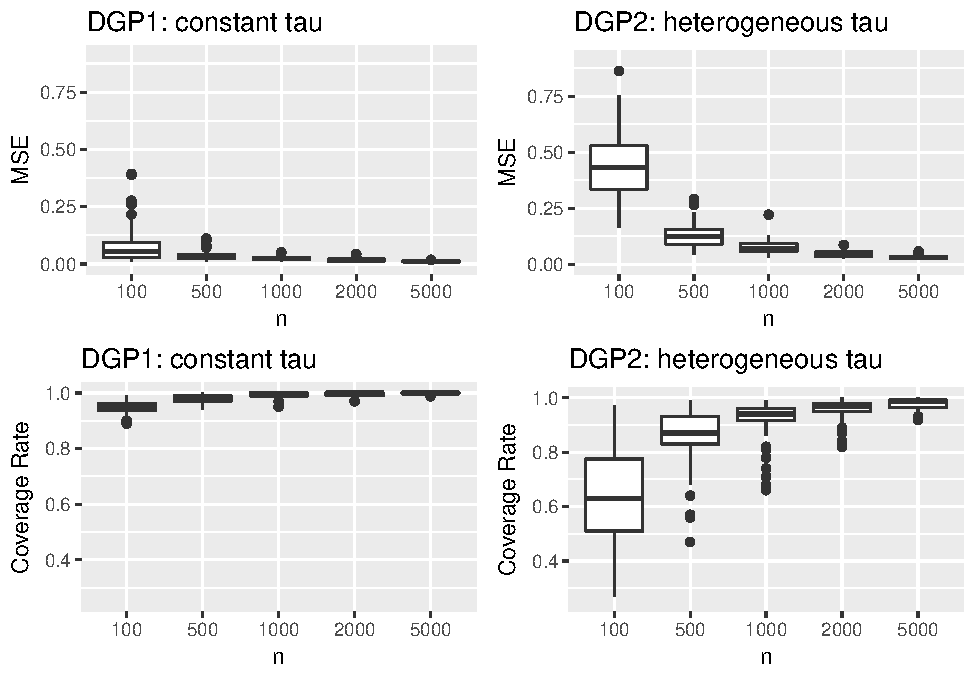
\includegraphics{report_files/figure-latex/fig1-1} \caption{\label{fig:fig1}MSE and Coverage Rate with Different Sample Size n}\label{fig:fig1}
\end{figure}

Figure \ref{fig:fig1} displays the MSE and 95\% confidence interval
coverage rate. Under the data generating process of constant treatment
effect, the MSE decays very fast as sample size \(n\) increases. Under
the DGP of heterogeneous treatment effect, the MSE is slightly larger
and it decays slightly slower. When \(n\) is as large as 5000, we
achieve considerably small MSE.

Surprisingly, the confidence interval performs very well for the DGP of
constant \(\tau\). Even in small sample \(n=100\), the simulation
coverage rate achieves about 95\%. What is interesting is that the
confidence interval seems ``over-accurate'' for DGP1. In the case of
\(n=5000\), we obtain almost 100\% accuracy that the 95\% confidence
interval will always cover the true \(\tau\).

As for the DGP2, we need larger sample for the confidence coverage to
converge. When \(n=100\), in median the 95\% confidence interval
successfully covers the true \(\tau\) for only about 60\% of the time.
When \(n=1000\), the median coverage rate achieves 95\%. However, when
\(n=5000\), we have the ``over-accurate'' issue again.

\begin{figure}[h!]
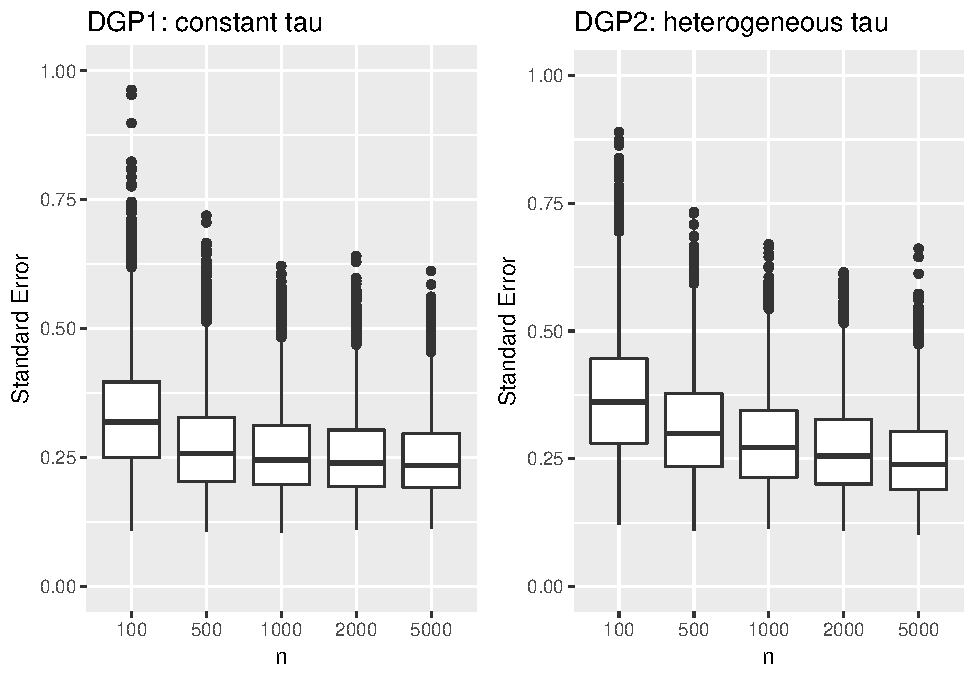
\includegraphics{report_files/figure-latex/fig2-1} \caption{\label{fig:fig2}Standard Errors with Different Sample Size n}\label{fig:fig2}
\end{figure}

In Figure \ref{fig:fig2} I plot the standard errors in the simulation.
We can see that the standard errors are pretty stable and have not
converged even when \(n=5000\). Theoretically, as sample size increases,
we should have smaller standard error for our estimator. But it is
clearly not the case here. Figure \ref{fig:fig1} has told us that the
MSE is shrinking and basically converges when \(n=5000\). In other
words, the point estimates are very close to the true value when
\(n=5000\). Therefore, I conjecture that the standard errors are ``too
large'' in large sample, and hence the 95\% confidence intervals are
``too wide'', which might lead us to the situation that, in hypothesis
testing we are less likely to reject than we should.

\begin{figure}[h]
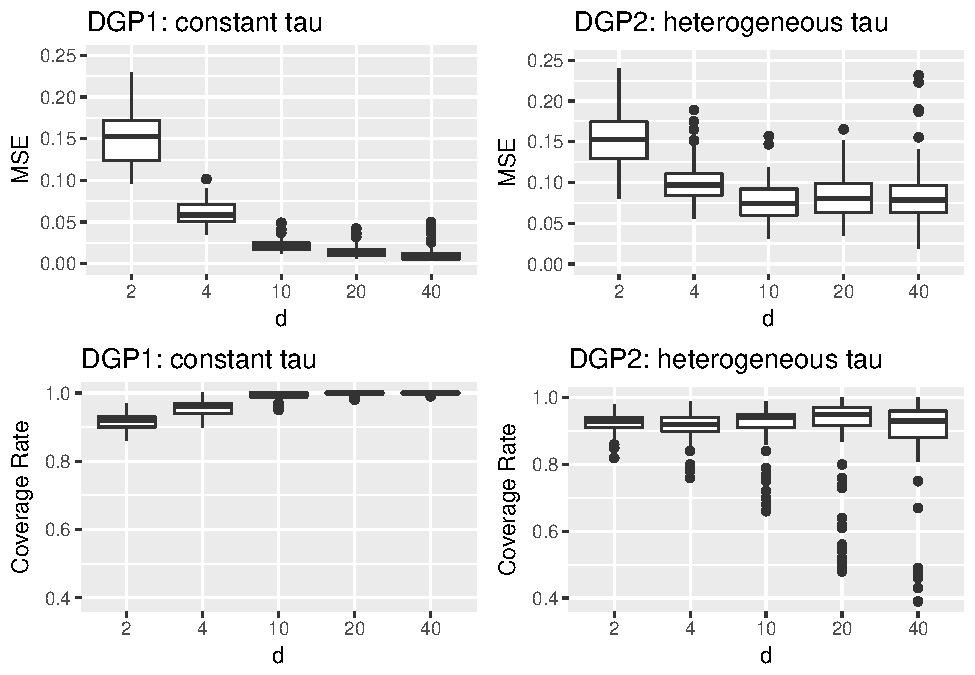
\includegraphics{report_files/figure-latex/fig3-1} \caption{\label{fig:fig3}MSE and Coverage Rate with Different Numbers of Covariates d}\label{fig:fig3}
\end{figure}

In both data generating processes, only the first two covariates \(X1\),
\(X2\) contribute to the \(\tau(\cdot)\) function. Therefore, adding
extra covariates is purely adding ``noise'' to the causal forest
algorithm. We should expect the variance of the heterogenous effect
estimates increases as \(d\) increases.

\subsubsection{Tuning Parameters}\label{tuning-parameters}

I try varying five tuning parameters, one at a time. I use DGP2 and fix
\(n=1000, d=10\)

\begin{enumerate}
\def\labelenumi{\arabic{enumi}.}
\tightlist
\item
  Sample fraction used in each tree training; (default 0.5)
\item
  Covariates used in each tree training; (default \(\frac{2}{3}d\))
\item
  Number of trees; (default 2000)
\item
  Minimun \# observations in each terminal node; (default NULL)
\item
  Regularization parameter \(\lambda\); (default 0)
\end{enumerate}

I Try sample fraction \(s = 0.1, 0.2, 0.3, 0.4, 0.5\)

\begin{longtable}[]{@{}ccc@{}}
\caption{MSE and Coverage Rate with Different Sample Fraction
s}\tabularnewline
\toprule
\begin{minipage}[b]{0.08\columnwidth}\centering\strut
s\strut
\end{minipage} & \begin{minipage}[b]{0.10\columnwidth}\centering\strut
MSE\strut
\end{minipage} & \begin{minipage}[b]{0.13\columnwidth}\centering\strut
coverage\strut
\end{minipage}\tabularnewline
\midrule
\endfirsthead
\toprule
\begin{minipage}[b]{0.08\columnwidth}\centering\strut
s\strut
\end{minipage} & \begin{minipage}[b]{0.10\columnwidth}\centering\strut
MSE\strut
\end{minipage} & \begin{minipage}[b]{0.13\columnwidth}\centering\strut
coverage\strut
\end{minipage}\tabularnewline
\midrule
\endhead
\begin{minipage}[t]{0.08\columnwidth}\centering\strut
0.1\strut
\end{minipage} & \begin{minipage}[t]{0.10\columnwidth}\centering\strut
0.242\strut
\end{minipage} & \begin{minipage}[t]{0.13\columnwidth}\centering\strut
0.535\strut
\end{minipage}\tabularnewline
\begin{minipage}[t]{0.08\columnwidth}\centering\strut
0.2\strut
\end{minipage} & \begin{minipage}[t]{0.10\columnwidth}\centering\strut
0.123\strut
\end{minipage} & \begin{minipage}[t]{0.13\columnwidth}\centering\strut
0.87\strut
\end{minipage}\tabularnewline
\begin{minipage}[t]{0.08\columnwidth}\centering\strut
0.3\strut
\end{minipage} & \begin{minipage}[t]{0.10\columnwidth}\centering\strut
0.082\strut
\end{minipage} & \begin{minipage}[t]{0.13\columnwidth}\centering\strut
0.92\strut
\end{minipage}\tabularnewline
\begin{minipage}[t]{0.08\columnwidth}\centering\strut
0.4\strut
\end{minipage} & \begin{minipage}[t]{0.10\columnwidth}\centering\strut
0.073\strut
\end{minipage} & \begin{minipage}[t]{0.13\columnwidth}\centering\strut
0.94\strut
\end{minipage}\tabularnewline
\begin{minipage}[t]{0.08\columnwidth}\centering\strut
0.5\strut
\end{minipage} & \begin{minipage}[t]{0.10\columnwidth}\centering\strut
0.075\strut
\end{minipage} & \begin{minipage}[t]{0.13\columnwidth}\centering\strut
0.94\strut
\end{minipage}\tabularnewline
\bottomrule
\end{longtable}

Try \# covariates in each tree training \(t = 4, 5, 6, 7, 8\)

\begin{longtable}[]{@{}ccc@{}}
\caption{MSE and Coverage Rate with Different Number of Training
Covariates t}\tabularnewline
\toprule
\begin{minipage}[b]{0.05\columnwidth}\centering\strut
t\strut
\end{minipage} & \begin{minipage}[b]{0.10\columnwidth}\centering\strut
MSE\strut
\end{minipage} & \begin{minipage}[b]{0.13\columnwidth}\centering\strut
coverage\strut
\end{minipage}\tabularnewline
\midrule
\endfirsthead
\toprule
\begin{minipage}[b]{0.05\columnwidth}\centering\strut
t\strut
\end{minipage} & \begin{minipage}[b]{0.10\columnwidth}\centering\strut
MSE\strut
\end{minipage} & \begin{minipage}[b]{0.13\columnwidth}\centering\strut
coverage\strut
\end{minipage}\tabularnewline
\midrule
\endhead
\begin{minipage}[t]{0.05\columnwidth}\centering\strut
4\strut
\end{minipage} & \begin{minipage}[t]{0.10\columnwidth}\centering\strut
0.102\strut
\end{minipage} & \begin{minipage}[t]{0.13\columnwidth}\centering\strut
0.865\strut
\end{minipage}\tabularnewline
\begin{minipage}[t]{0.05\columnwidth}\centering\strut
5\strut
\end{minipage} & \begin{minipage}[t]{0.10\columnwidth}\centering\strut
0.082\strut
\end{minipage} & \begin{minipage}[t]{0.13\columnwidth}\centering\strut
0.92\strut
\end{minipage}\tabularnewline
\begin{minipage}[t]{0.05\columnwidth}\centering\strut
6\strut
\end{minipage} & \begin{minipage}[t]{0.10\columnwidth}\centering\strut
0.079\strut
\end{minipage} & \begin{minipage}[t]{0.13\columnwidth}\centering\strut
0.92\strut
\end{minipage}\tabularnewline
\begin{minipage}[t]{0.05\columnwidth}\centering\strut
7\strut
\end{minipage} & \begin{minipage}[t]{0.10\columnwidth}\centering\strut
0.07\strut
\end{minipage} & \begin{minipage}[t]{0.13\columnwidth}\centering\strut
0.94\strut
\end{minipage}\tabularnewline
\begin{minipage}[t]{0.05\columnwidth}\centering\strut
8\strut
\end{minipage} & \begin{minipage}[t]{0.10\columnwidth}\centering\strut
0.074\strut
\end{minipage} & \begin{minipage}[t]{0.13\columnwidth}\centering\strut
0.94\strut
\end{minipage}\tabularnewline
\bottomrule
\end{longtable}

Try \# trees \(b = 500, 1000, 2000, 4000, 6000\)

\begin{longtable}[]{@{}ccc@{}}
\toprule
\begin{minipage}[b]{0.09\columnwidth}\centering\strut
b\strut
\end{minipage} & \begin{minipage}[b]{0.10\columnwidth}\centering\strut
MSE\strut
\end{minipage} & \begin{minipage}[b]{0.13\columnwidth}\centering\strut
coverage\strut
\end{minipage}\tabularnewline
\midrule
\endhead
\begin{minipage}[t]{0.09\columnwidth}\centering\strut
500\strut
\end{minipage} & \begin{minipage}[t]{0.10\columnwidth}\centering\strut
0.088\strut
\end{minipage} & \begin{minipage}[t]{0.13\columnwidth}\centering\strut
0.97\strut
\end{minipage}\tabularnewline
\begin{minipage}[t]{0.09\columnwidth}\centering\strut
1000\strut
\end{minipage} & \begin{minipage}[t]{0.10\columnwidth}\centering\strut
0.079\strut
\end{minipage} & \begin{minipage}[t]{0.13\columnwidth}\centering\strut
0.96\strut
\end{minipage}\tabularnewline
\begin{minipage}[t]{0.09\columnwidth}\centering\strut
2000\strut
\end{minipage} & \begin{minipage}[t]{0.10\columnwidth}\centering\strut
0.076\strut
\end{minipage} & \begin{minipage}[t]{0.13\columnwidth}\centering\strut
0.95\strut
\end{minipage}\tabularnewline
\begin{minipage}[t]{0.09\columnwidth}\centering\strut
4000\strut
\end{minipage} & \begin{minipage}[t]{0.10\columnwidth}\centering\strut
0.077\strut
\end{minipage} & \begin{minipage}[t]{0.13\columnwidth}\centering\strut
0.94\strut
\end{minipage}\tabularnewline
\begin{minipage}[t]{0.09\columnwidth}\centering\strut
6000\strut
\end{minipage} & \begin{minipage}[t]{0.10\columnwidth}\centering\strut
0.075\strut
\end{minipage} & \begin{minipage}[t]{0.13\columnwidth}\centering\strut
0.915\strut
\end{minipage}\tabularnewline
\bottomrule
\end{longtable}

Try minimun node size = 0, 10, 20, 40, 80

\begin{longtable}[]{@{}ccc@{}}
\toprule
\begin{minipage}[b]{0.09\columnwidth}\centering\strut
size\strut
\end{minipage} & \begin{minipage}[b]{0.10\columnwidth}\centering\strut
MSE\strut
\end{minipage} & \begin{minipage}[b]{0.13\columnwidth}\centering\strut
coverage\strut
\end{minipage}\tabularnewline
\midrule
\endhead
\begin{minipage}[t]{0.09\columnwidth}\centering\strut
0\strut
\end{minipage} & \begin{minipage}[t]{0.10\columnwidth}\centering\strut
0.068\strut
\end{minipage} & \begin{minipage}[t]{0.13\columnwidth}\centering\strut
0.94\strut
\end{minipage}\tabularnewline
\begin{minipage}[t]{0.09\columnwidth}\centering\strut
10\strut
\end{minipage} & \begin{minipage}[t]{0.10\columnwidth}\centering\strut
0.066\strut
\end{minipage} & \begin{minipage}[t]{0.13\columnwidth}\centering\strut
0.89\strut
\end{minipage}\tabularnewline
\begin{minipage}[t]{0.09\columnwidth}\centering\strut
20\strut
\end{minipage} & \begin{minipage}[t]{0.10\columnwidth}\centering\strut
0.066\strut
\end{minipage} & \begin{minipage}[t]{0.13\columnwidth}\centering\strut
0.9\strut
\end{minipage}\tabularnewline
\begin{minipage}[t]{0.09\columnwidth}\centering\strut
40\strut
\end{minipage} & \begin{minipage}[t]{0.10\columnwidth}\centering\strut
0.063\strut
\end{minipage} & \begin{minipage}[t]{0.13\columnwidth}\centering\strut
0.915\strut
\end{minipage}\tabularnewline
\begin{minipage}[t]{0.09\columnwidth}\centering\strut
80\strut
\end{minipage} & \begin{minipage}[t]{0.10\columnwidth}\centering\strut
0.076\strut
\end{minipage} & \begin{minipage}[t]{0.13\columnwidth}\centering\strut
0.905\strut
\end{minipage}\tabularnewline
\bottomrule
\end{longtable}

Try \(\lambda = 0.1, 1, 5, 10, 100\)

\begin{longtable}[]{@{}ccc@{}}
\toprule
\begin{minipage}[b]{0.11\columnwidth}\centering\strut
lambda\strut
\end{minipage} & \begin{minipage}[b]{0.10\columnwidth}\centering\strut
MSE\strut
\end{minipage} & \begin{minipage}[b]{0.13\columnwidth}\centering\strut
coverage\strut
\end{minipage}\tabularnewline
\midrule
\endhead
\begin{minipage}[t]{0.11\columnwidth}\centering\strut
0\strut
\end{minipage} & \begin{minipage}[t]{0.10\columnwidth}\centering\strut
0.067\strut
\end{minipage} & \begin{minipage}[t]{0.13\columnwidth}\centering\strut
0.95\strut
\end{minipage}\tabularnewline
\begin{minipage}[t]{0.11\columnwidth}\centering\strut
0.1\strut
\end{minipage} & \begin{minipage}[t]{0.10\columnwidth}\centering\strut
0.069\strut
\end{minipage} & \begin{minipage}[t]{0.13\columnwidth}\centering\strut
0.94\strut
\end{minipage}\tabularnewline
\begin{minipage}[t]{0.11\columnwidth}\centering\strut
1\strut
\end{minipage} & \begin{minipage}[t]{0.10\columnwidth}\centering\strut
0.066\strut
\end{minipage} & \begin{minipage}[t]{0.13\columnwidth}\centering\strut
0.94\strut
\end{minipage}\tabularnewline
\begin{minipage}[t]{0.11\columnwidth}\centering\strut
5\strut
\end{minipage} & \begin{minipage}[t]{0.10\columnwidth}\centering\strut
0.076\strut
\end{minipage} & \begin{minipage}[t]{0.13\columnwidth}\centering\strut
0.925\strut
\end{minipage}\tabularnewline
\begin{minipage}[t]{0.11\columnwidth}\centering\strut
10\strut
\end{minipage} & \begin{minipage}[t]{0.10\columnwidth}\centering\strut
0.079\strut
\end{minipage} & \begin{minipage}[t]{0.13\columnwidth}\centering\strut
0.92\strut
\end{minipage}\tabularnewline
\bottomrule
\end{longtable}


\end{document}
